\section{Tensor Flow}

Para la implementación en Tensor Flow se utilizó una red neuronal sencilla con 2 neuronas de entrada, 5 neuronas en la capa oculta y 1 neurona en la capa de salida. La Figura \ref{fig:RedTF} muestra esta red.

\begin{figure}[H]
    \centering
    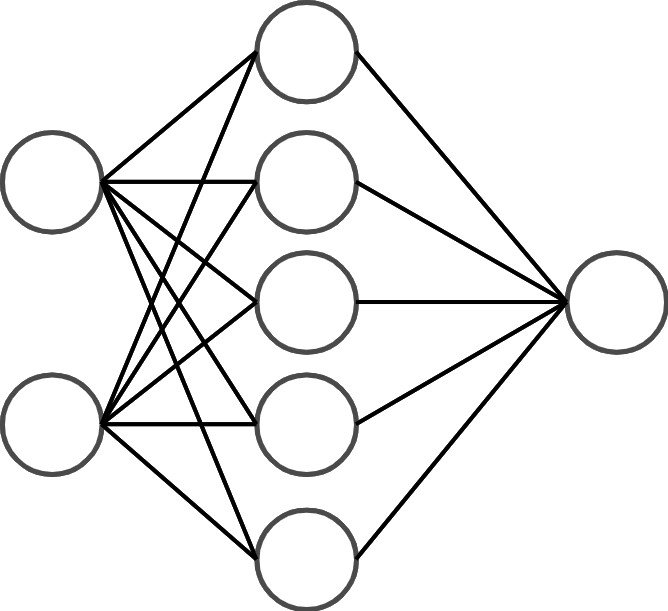
\includegraphics[width=0.5\textwidth]{Resultados/imgs/RedTF.png}
    \caption{Red neuronal implementada en Tensor Flow.}
    \label{fig:RedTF}
\end{figure}

Para la implementación con la biblioteca Tensor Flow se realizaron 1000 entrenamientos ya que esta es la cantidad máxima permitida por los recursos del hardware utilizado, con los resultados de estos entrenamientos se obtuvo el valor mínimo el valor máximo y el promedio de todos los experimentos.

\subsection{Carril central}

La Tabla \ref{tab:resultadosTFCCentral} muestra los resultados para el carril central en kilómetros por hora, podemos notar que para estos experimentos tenemos un promedio de 12.762 K/H con un valor mínimo de 1.872 K/H.


\begin{table}[H]
    \centering
    \caption{Resultados utilizando Tensor Flow Carril Central}
    \label{tab:resultadosTFCCentral}
    \begin{tabular}{|c|l|} \hline

    & \multicolumn{1}{c|}{\textbf{Error}} \\ \hline
    \textbf{MIN} & 1.872 \\ \hline
    \textbf{MAX} & 237.067 \\ \hline
    \textbf{Promedio} & 12.762 \\ \hline
    \end{tabular}
\end{table}


\subsection{Ultimo Carril}

La Tabla \ref{tab:resultadosTFCUltimo} muestra los resultados para el ultimo carril en kilómetros por hora, la cual nos muestra un valor mínimo de 2.128 K/H con un promedio de 13.172 K/H.


\begin{table}[H]
    \centering
    \caption{Resultados utilizando Tensor Flow Ultimo Carril}
    \label{tab:resultadosTFCUltimo}
    \begin{tabular}{|c|l|}\hline

    & \multicolumn{1}{c|}{\textbf{Error}} \\ \hline
    \textbf{MIN} & 2.128 \\ \hline
    \textbf{MAX} & 253.930 \\ \hline
    \textbf{Promedio} & 13.172 \\ \hline
    \end{tabular}
\end{table}
